% This file contains the TikZ source code for generating two
% of the diagrams in the LearnSAT tutorial
% The PDF files output when formatted are used in the tutorial
% This is done so that the tutorial can be modified
% by people who lack experience in TikZ
% and don't want to install the package

\documentclass[11pt]{article}
\usepackage{tikz}
\usetikzlibrary{external,shapes.geometric}
\tikzexternalize[prefix=tikz/]

% Style for displaying labels in the diagrams
\newcommand*{\p}[1]{\textsf{\Large #1}}

\begin{document}

% Example showing that the third Ramsey number is greater than 5
% The complete graph K_5 can be colored in two colors so that no
% triangle is monochromatic
% Both colors and line styles are used so that the diagram is readable
% when printed or by people with deficiencies in their color perception
\begin{center}
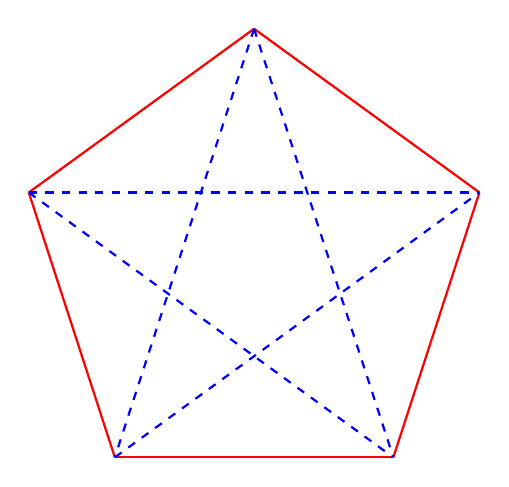
\begin{tikzpicture}
\node (pentagon) [minimum size=6cm,regular polygon,regular polygon sides=5] at (0,0) {};
\draw[thick,red] (pentagon.corner 1) -- (pentagon.corner 2);
\draw[thick,red] (pentagon.corner 2) -- (pentagon.corner 3);
\draw[thick,red] (pentagon.corner 3) -- (pentagon.corner 4);
\draw[thick,red] (pentagon.corner 4) -- (pentagon.corner 5);
\draw[thick,red] (pentagon.corner 5) -- (pentagon.corner 1);
\draw[thick,blue,dashed] (pentagon.corner 1) -- (pentagon.corner 3);
\draw[thick,blue,dashed] (pentagon.corner 1) -- (pentagon.corner 4);
\draw[thick,blue,dashed] (pentagon.corner 2) -- (pentagon.corner 4);
\draw[thick,blue,dashed] (pentagon.corner 2) -- (pentagon.corner 5);
\draw[thick,blue,dashed] (pentagon.corner 3) -- (pentagon.corner 5);
\end{tikzpicture}
\end{center}

% McGregor graph of order 3 for graph coloring
\begin{center}
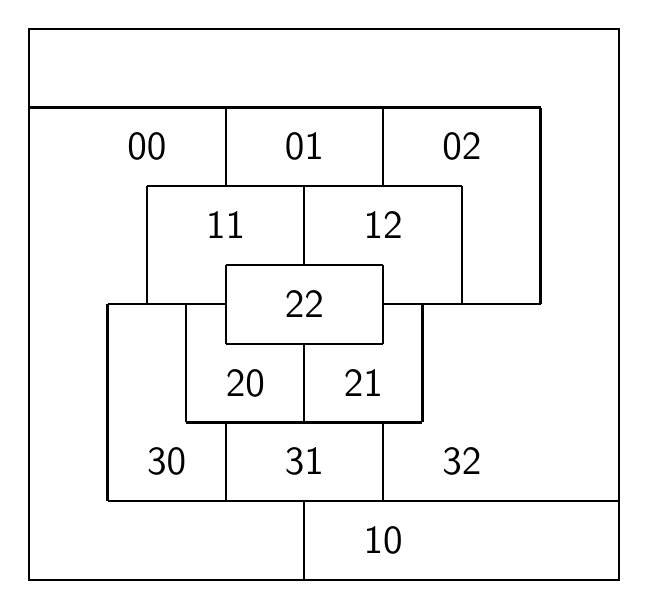
\begin{tikzpicture}[scale=.5]
\draw[thick] (0,0) rectangle +(15,14);

\draw[thick] (2,2) -- (15,2);
\draw[thick] (4,4) -- (10,4);
\draw[thick] (5,6) -- (9,6);
\draw[thick] (5,8) -- (9,8);
\draw[thick] (2,7) -- (5,7);
\draw[thick] (9,7) -- (13,7);
\draw[thick] (3,10) -- (11,10);
\draw[thick] (0,12) -- (13,12);

\draw[thick] (7,0) -- (7,2);
\draw[thick] (2,2) -- (2,7);
\draw[thick] (4,4) -- (4,7);
\draw[thick] (5,2) -- (5,4);
\draw[thick] (9,2) -- (9,4);
\draw[thick] (7,4) -- (7,6);
\draw[thick] (5,6) -- (5,8);
\draw[thick] (9,6) -- (9,8);
\draw[thick] (9,2) -- (9,4);
\draw[thick] (10,4) -- (10,7);
\draw[thick] (3,7) -- (3,10);
\draw[thick] (7,8) -- (7,10);
\draw[thick] (11,7) -- (11,10);
\draw[thick] (13,7) -- (13,12);
\draw[thick] (5,10) -- (5,12);
\draw[thick] (9,10) -- (9,12);

\node at (3,11) {\p{00}};
\node at (7,11) {\p{01}};
\node at (11,11) {\p{02}};
\node at (9,1) {\p{10}};
\node at (5,9) {\p{11}};
\node at (9,9) {\p{12}};
\node at (5.5,5) {\p{20}};
\node at (8.5,5) {\p{21}};
\node at (7,7) {\p{22}};
\node at (3.5,3) {\p{30}};
\node at (7,3) {\p{31}};
\node at (11,3) {\p{32}};
\end{tikzpicture}

\end{center}


\end{document}
